\documentclass[twoside,a4paper]{article}
\usepackage{geometry}
\geometry{margin=1.5cm, vmargin={0pt,1cm}}
\setlength{\topmargin}{-1cm}
\setlength{\paperheight}{29.7cm}
\setlength{\textheight}{25.3cm}

% useful packages.
\usepackage{amsfonts}
\usepackage{amsmath}
\usepackage{amssymb}
\usepackage{amsthm}
\usepackage{enumerate}
\usepackage{graphicx}
\usepackage{multicol}
\usepackage{fancyhdr}
\usepackage{layout}
\usepackage{float}
% some common command
\newcommand{\dif}{\mathrm{d}}
\newcommand{\avg}[1]{\left\langle #1 \right\rangle}
\newcommand{\difFrac}[2]{\frac{\dif #1}{\dif #2}}
\newcommand{\pdfFrac}[2]{\frac{\partial #1}{\partial #2}}
\newcommand{\OFL}{\mathrm{OFL}}
\newcommand{\UFL}{\mathrm{UFL}}
\newcommand{\fl}{\mathrm{fl}}
\newcommand{\op}{\odot}
\newcommand{\Eabs}{E_{\mathrm{abs}}}
\newcommand{\Erel}{E_{\mathrm{rel}}}

\begin{document}

\pagestyle{fancy}
\fancyhead{}
\lhead{Jovi Wong(3180104829)}
\chead{Numerical Analysis homework \#7}
\rhead{2020/5/18}


\section*{I. Can we compute root with absolute accuracy$<10^{-6}$ by bisection method}
No, we can't. Because $128=(10000000)_2=(1.0000000)_2\times2^{7}$ takes up $8$ digits within $24$ digits. As a result, the minimum number can be denoted is $min=2^{7-23}=2^{-16}\approx15.26\times10^{-6}$ so that $\epsilon_u = \frac{min}{2}=7.63\times10^{-6}>10^{-6}$. In other word, we can't compute roots with absolute accuracy $<10^{-6}$ .

\section*{II. What are condition numbers of following functions?Where are they large?}
\subsection*{a. $(x-1)^\alpha$,}
$cond_f(x)=|\frac{\alpha x(x-1)^{\alpha-1}}{(x-1)^\alpha}|=|\frac{\alpha x}{x-1}|$, when $x\to1$, $cond_f(x)\to\infty$
\subsection*{b. $\ln{x}$ ,}
$cond_f(x)=|\frac{x\cdot\frac{1}{x}}{\ln{x}}|=|\frac{1}{\ln{x}}|$ , when $x\to1$, $cond_f(x)\to\infty$
\subsection*{c. $e^{x}$ ,}
$cond_f(x)=|\frac{xe^x}{e^x}|=|x|$ , when $x\to\infty$, $cond_f(x)\to\infty$
\subsection*{d. $\arccos{x}$}
$cond_f(x)=|\frac{x}{\sqrt{1-x^2}\arccos{x}}|$ , when $x\to 1$ or $x\to-1$, $cond_f(x)\to\infty$ 
\section*{III. Repeat Example 1.25 for $f(x)=\frac{\sin{x}}{1+\cos{x}}$ on $(0,\frac{\pi}{2})$}
We can know that
\begin{gather}
f'(x)=\frac{1}{1+\cos{x}}\\
cond_f(x)=|\frac{x}{\sin{x}}|
\end{gather}
By theorem 1.29, 
\begin{gather}
f_A(x)=\frac{(1+\delta_1)\sin{x}}{(1+\delta_3)(1+(1+\delta_2)\cos{x})}(1+\delta_4)\\
=\frac{\sin{x}}{1+\cos{x}}(1+\delta_1+\delta_4-\delta_3-\frac{\delta_2\cos{x}}{1+(1+\delta_2)\cos{x}})
\end{gather}
where $|\delta_i|<\epsilon_u$ , consequently, $\varphi(x)=3+\frac{\cos{x}}{1+cos{x}}$. Finally,
\begin{gather}
cond_A(x)\leq\frac{\sin{x}}{x}(3+\frac{\cos{x}}{1+\cos{x}})
\end{gather}


\section*{IV. Consider function $f(x)=1-e^{-x}$ for $x\in[0,1]$}
\subsection*{a. Show that $cond_f(x)\leq 1$ for $x\in[0,1]$}
Because $cond_f(x)=|\frac{xe^{-x}}{1-e^{-x}}|=\frac{x}{e^x-1}$ on $(0,1]$ and $cond_f(0)=1$ by L'Hospital theorem. Besides, we know that $e^x>1+x$, therefore, $cond_f(x) < 1$ on $(0,1]$ and  $cond_f(x) \leq 1$ on $[0,1]$. Hence proved.
\subsection*{b. Estimate $cond_{A}(x)$ for $x\in[0,1]$}
We can know that
\begin{gather}
f_A(x)=(1+\delta_2)(1-(1+\delta_1)e^{-x})\\
=(1-e^{-x})(1+\delta_1+\delta_2+\delta_1\delta_2-\frac{\delta_1(1+\delta_2)}{1-e^{-x}})
\end{gather}
where $|\delta_i|<\epsilon_u$ , consequently, $\varphi(x)=2+\frac{1}{1-e^{-x}}$ . Therefore, for $x\in(0,1]$
\begin{gather}
cond_A(x)\leq \frac{e^x-1}{x}(2+\frac{1}{1-e^{-x}})
\end{gather}

\subsection*{c. Plot $cond_f(x)$ and $cond_A(x)$ as function of $x$ on $[0,1]$}
\begin{figure}[H]
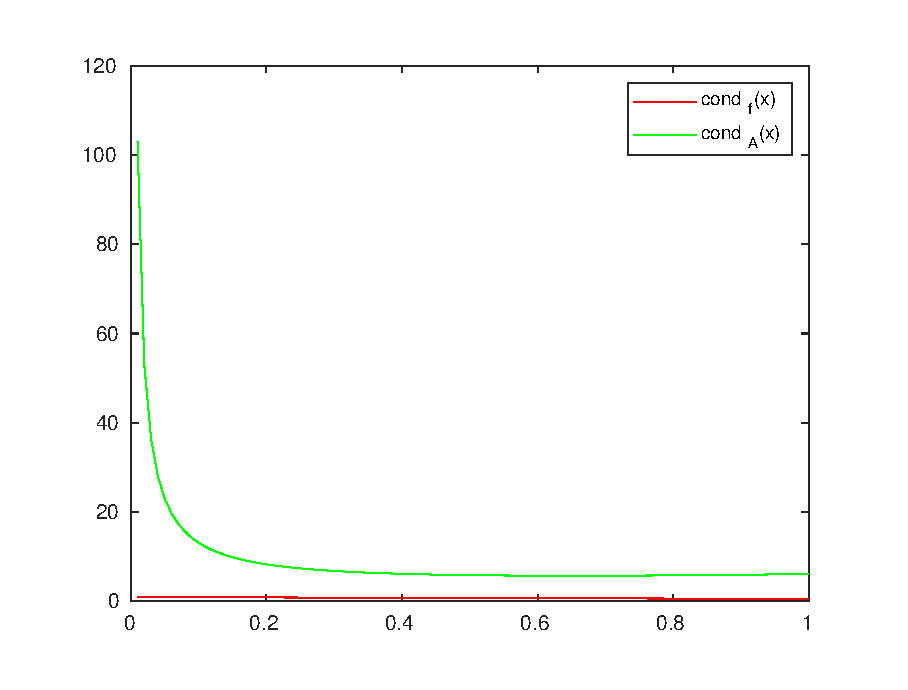
\includegraphics[width=5in]{./figure/comparison.eps}
\caption{comparison between $cond_f(x)$ and $cond_A(x)$}
\end{figure}

\begin{figure}[H]
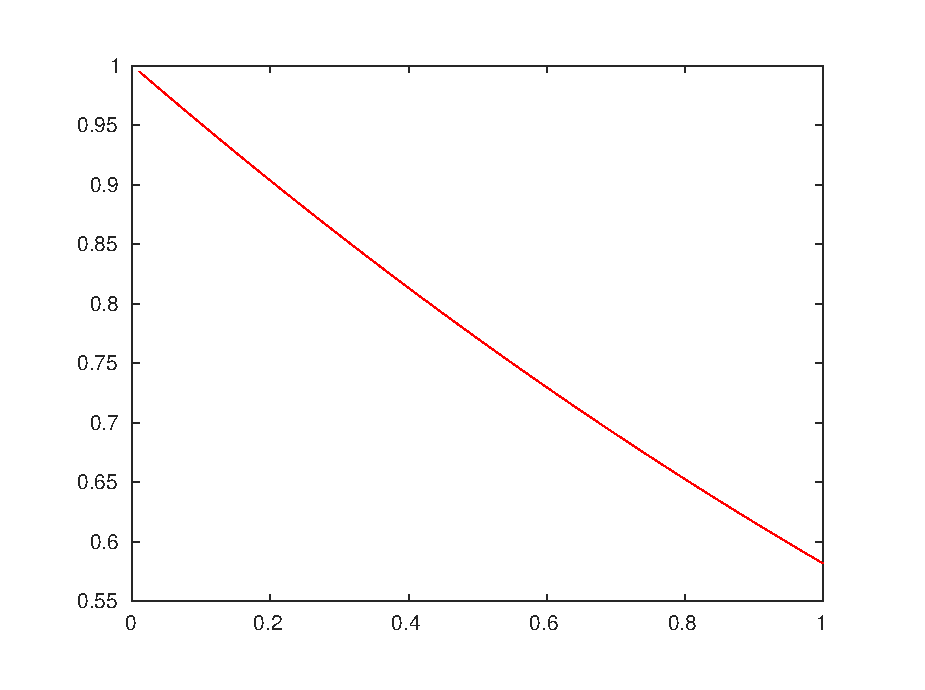
\includegraphics[width=5in]{./figure/condf.eps}
\caption{$cond_f(x)$}
\end{figure}
These two figures differ from each other totally. I think one of reasons is that $cond_A$ figure just shows a upper bound rather than explicit expression. Besides, relative error of $f_A\to\infty$ when $x\to0^+$, so $cond_A\to\infty$ as result.
\section*{V. For Wilkinson example, compute condition number and compare result}
Assume $q(r)=0$, namely,
\begin{gather}
q(r)=a_0+a_1r+\cdots+a_{n-1}r^{n-1}+r^n=0
\end{gather}
We can take equation as a function $f$ of $a_i$, denoted by
\begin{gather}
r=f(a_0,a_1,\cdots,a_{n-1})
\end{gather}
Also, let $F(a_0,a_1,\cdots,a_{n-1},r)=f(a_0,a_1,\cdots,a_{n-1})-r$ . Consequently, we can get
\begin{gather}
\frac{\partial r}{\partial a_i}=-\frac{r^i}{a_1+2a_2r+\cdots+(n-1)a_{n-1}r^{n-2}+nr^{n-1}}
\end{gather}
by
\begin{gather}
\frac{\partial{F}}{\partial{r}}=a_1+2a_2r+\cdots+(n-1)a_{n-1}r^{n-2}+nr^{n-1}\\
\frac{\partial{F}}{\partial{a_i}}=x^{i}, \forall i = 0,1,\cdots,n-1\\
\frac{\partial r}{\partial a_i}=-\frac{\frac{\partial{F}}{\partial{a_i}}}{\frac{\partial{F}}{\partial{r}}}
\end{gather}
According to definition 1.45, let $cond_f(\overrightarrow{x}) = ||A(\overrightarrow{x})||$ , where $A=[a_{1i}(\overrightarrow{x})]$ , $\overrightarrow{x}=(a_0,a_1,\cdots,a_{n-1})$. To be specific,
\begin{gather}
a_{1i}(\overrightarrow{x})=|\frac{x_i\frac{\partial f}{\partial x_i}}{f(\overrightarrow{x})}|=|\frac{a_i}{r}\frac{\partial r}{\partial a_i}|=|\frac{a_ir^{i-1}}{a_1+2a_2r+\cdots+(n-1)a_{n-1}r^{n-2}+nr^{n-1}}|
\end{gather}
Therefore,
\begin{gather}
cond_f(\overrightarrow{x})=||A(\overrightarrow{x})||=\max_{0 \leq i \leq {n-1}}|\frac{a_ir^{i-1}}{a_1+2a_2r+\cdots+(n-1)a_{n-1}r^{n-2}+nr^{n-1}}|\\
=\max_{0 \leq i \leq {n-1}} \{ |a_ir^{i-1}| \} |\frac{1}{a_1+2a_2r+\cdots+(n-1)a_{n-1}r^{n-2}+nr^{n-1}}|
\end{gather}
As for Wilkinson Example, namely , take $f(x)= \prod_{k=1}^{p}(x-k)$ into (17) and we can know that
\begin{gather}
cond_f(\overrightarrow{x})=|\frac{p^{n-2}}{a_1+2a_2p+\cdots+(n-1)a_{n-1}p^{n-2}+np^{n-1}}|
\end{gather}  
The comparison reveals that conponentwise condition number of vector function is a better way to measure how is a function sensitive to variation than condition number.
\end{document}

%%% Local Variables: 
%%% mode: latex
%%% TeX-master: t
%%% End: 
